\documentclass[twoside,11pt]{article}

% Any additional packages needed should be included after jmlr2e.
% Note that jmlr2e.sty includes epsfig, amssymb, natbib and graphicx,
% and defines many common macros, such as 'proof' and 'example'.
%
% It also sets the bibliographystyle to plainnat; for more information on
% natbib citation styles, see the natbib documentation, a copy of which
% is archived at http://www.jmlr.org/format/natbib.pdf

% Available options for package jmlr2e are:
%
%   - abbrvbib : use abbrvnat for the bibliography style
%   - nohyperref : do not load the hyperref package
%   - preprint : remove JMLR specific information from the template,
%         useful for example for posting to preprint servers.
%
% Example of using the package with custom options:
%
%\usepackage[abbrvbib, preprint]{jmlr2e}
\usepackage[utf8]{inputenc}
\usepackage[T1]{fontenc}
\usepackage{jmlr2e}
\usepackage{booktabs}
\usepackage{hyperref}
\usepackage{graphicx}
%\usepackage{float}
\usepackage{placeins}


% Definitions of handy macros can go here
\newcommand{\dataset}{{\cal D}}
\newcommand{\fracpartial}[2]{\frac{\partial #1}{\partial  #2}}
\usepackage{xcolor}
\definecolor{diffcolor}{rgb}{0.16, 0.32, 0.75}
\newcommand{\diff}[1]{\textcolor{diffcolor}{#1}}

% Heading arguments are {volume}{year}{pages}{date submitted}{date published}{paper id}{author-full-names}
\usepackage{lastpage}
\jmlrheading{}{2026}{1-10}{}{}{}{}

% Short headings should be running head and authors last names
\ShortHeadings{Identity Framing in SLM Debates}{Rakowski, Czarnecki, Grabowski, Brandt}
\firstpageno{1}

\begin{document}

\title{
Identity-Induced Reasoning: How Ethnic and National Framing Affects Debate Outcomes in Small LLM Multi-Agent Systems
}

\author{\name Antoni Rakowski \email antoni.rakowski.stud@pw.edu.pl \\
    \name Ryszard Czarnecki \email ryszard.czarnecki.stud@pw.edu.pl \\
    \name Gabriel Grabowski \email gabriel.grabowski.stud@pw.edu.pl \\
    \name Aleksander Brandt \email aleksander.brandt.stud@pw.edu.pl \\
    \addr Warsaw University of Technology, Poland\\
}

\maketitle

\begin{abstract}%
We present a controlled study of small language models (SLMs) in multi-agent debates on historically, religiously, and geopolitically sensitive topics. Each agent is embodied via system-prompt personas representing specific national, ethnic, or religious identities, and evaluated across a factorial design crossing three prompt structures (plain user-turn, strict adversarial constraints, formal system prefix), two peer-awareness levels (whether an agent knows its opponent's identity), and three speaking-order permutations. Across 968 debates spanning eight model variants, we show that identity assignment dictates both semantic diversity and topic adherence, while content censorship operates at the model level rather than the persona level. We further identify \textit{Puppeteering}---a novel failure mode in which an agent abandons turn-taking boundaries and unilaterally scripts dialogue for both sides---as a systematic artifact of forum-based finetuning. Strict in-text constraints intended to prevent Puppeteering paradoxically \emph{exacerbate} it (the Backfire Effect), a formal system prefix is the only reliable mitigation, and Puppeteering degrades debate quality: lexical diversity collapses by $48\%$ (Cohen's $d = -1.44$, $p < 0.001$) while redundancy triples. These findings establish Puppeteering as a measurable, reproducible failure mode with direct implications for multi-agent system design.
\end{abstract}

\section{Introduction}

Small Language Models increasingly run locally on consumer hardware, yet many are fine-tuned on data and norms of a single language community, raising questions about culturally-specific framing. We investigate three questions: (i)~whether SLMs of different cultural training origin discuss controversial topics comparably under matched personas; (ii)~whether peer awareness changes agent behaviour; and (iii)~whether speaking order affects debate outcomes. Prior persona-effect studies \citep{salewski2023, deshpande2023} evaluate one model at a time, multi-agent debate \citep{du2023} targets factual reasoning rather than sensitive content, and bias surveys \citep{navigli2023} catalogue biases without cross-model comparison. We close this gap with a controlled head-to-head comparison across cultural framing, peer awareness, and speaking order.

\section{Methodology}

All experiments follow a \textbf{round-robin} protocol. Each debate consists of $3$ rounds of alternating responses. Each debate is repeated across $30$ seeds to account for sampling stochasticity.
We experiment with the following small open-source language models: \textit{Qwen 2.5 1.5B}, \textit{Qwen 2.5 1.5B (uncensored)}, \textit{Qwen 2.5 3B-Instruct (RLHF/SFT)}, \textit{Gemma 3 1B}, \textit{Gemma 3 1B (uncensored)}, \textit{Llama 3.2 1B}, \textit{Llama 3.2 1B (uncensored)}, \textit{Bielik 1.5B}. 

We measure the following dimensions of agent behaviour:
\textit{Semantic diversity (rule-based)}, \textit{Distinct-1 (lexical uniqueness)}, \textit{Topic Adherence (zero-shot via facebook/bart-large-mnli)}, \textit{Stereotyping Score (valurank/distilroberta-bias)}, \textit{Sentiment Flips (persuasion rate)}, \textit{Hostility (s-nlp/roberta-toxicity-classifier)}, \textit{Identity Bleed (Persona Boundary Violation)}, \textit{negative sentiment (cardiffnlp/twitter-roberta-base-sentiment-latest)}, \textit{anger}, and \textit{disgust}.

\section{Experiments}

We test agent behaviour across a range of national, ethnic and religious identities, grouped into categories based on the nature of the intergroup relationship.

\subsection{Groups with Historical Conflict}

All agents in this category debated the following topic: \textit{``Should countries allow diaspora communities to teach their own version of history to children in schools?''}

\subsubsection{Identity-Aware Condition}
We select pairs of nationalities with well-documented histories of political or military conflict: Israel--Palestine, Turkey--Armenia, and Tutsi--Hutu, with Ireland--Portugal serving as a neutral baseline. In this condition, each agent is explicitly informed of their opponent's assigned nationality via the system prompt.

\paragraph{Results.}
The effect of conflict identity on emotional and sentiment metrics varies substantially across models. Llama~3.2~1B exhibits the clearest identity-driven amplification: negative sentiment, anger, and disgust rise markedly for Israel/Palestine and Tutsi/Hutu relative to the baseline, while Turkey/Armenia produces a weaker effect. Llama~3.2~1B (uncensored) displays elevated emotional scores even at baseline, making conflict-specific effects difficult to isolate. Gemma~3~1B (uncensored) remains largely stable across conditions, indicating effective suppression of identity-induced affect. Qwen~2.5~1.5B shows mild elevations in negative sentiment and disgust on conflict pairs while remaining stable in anger.

\begin{figure}[htbp]
    \centering
    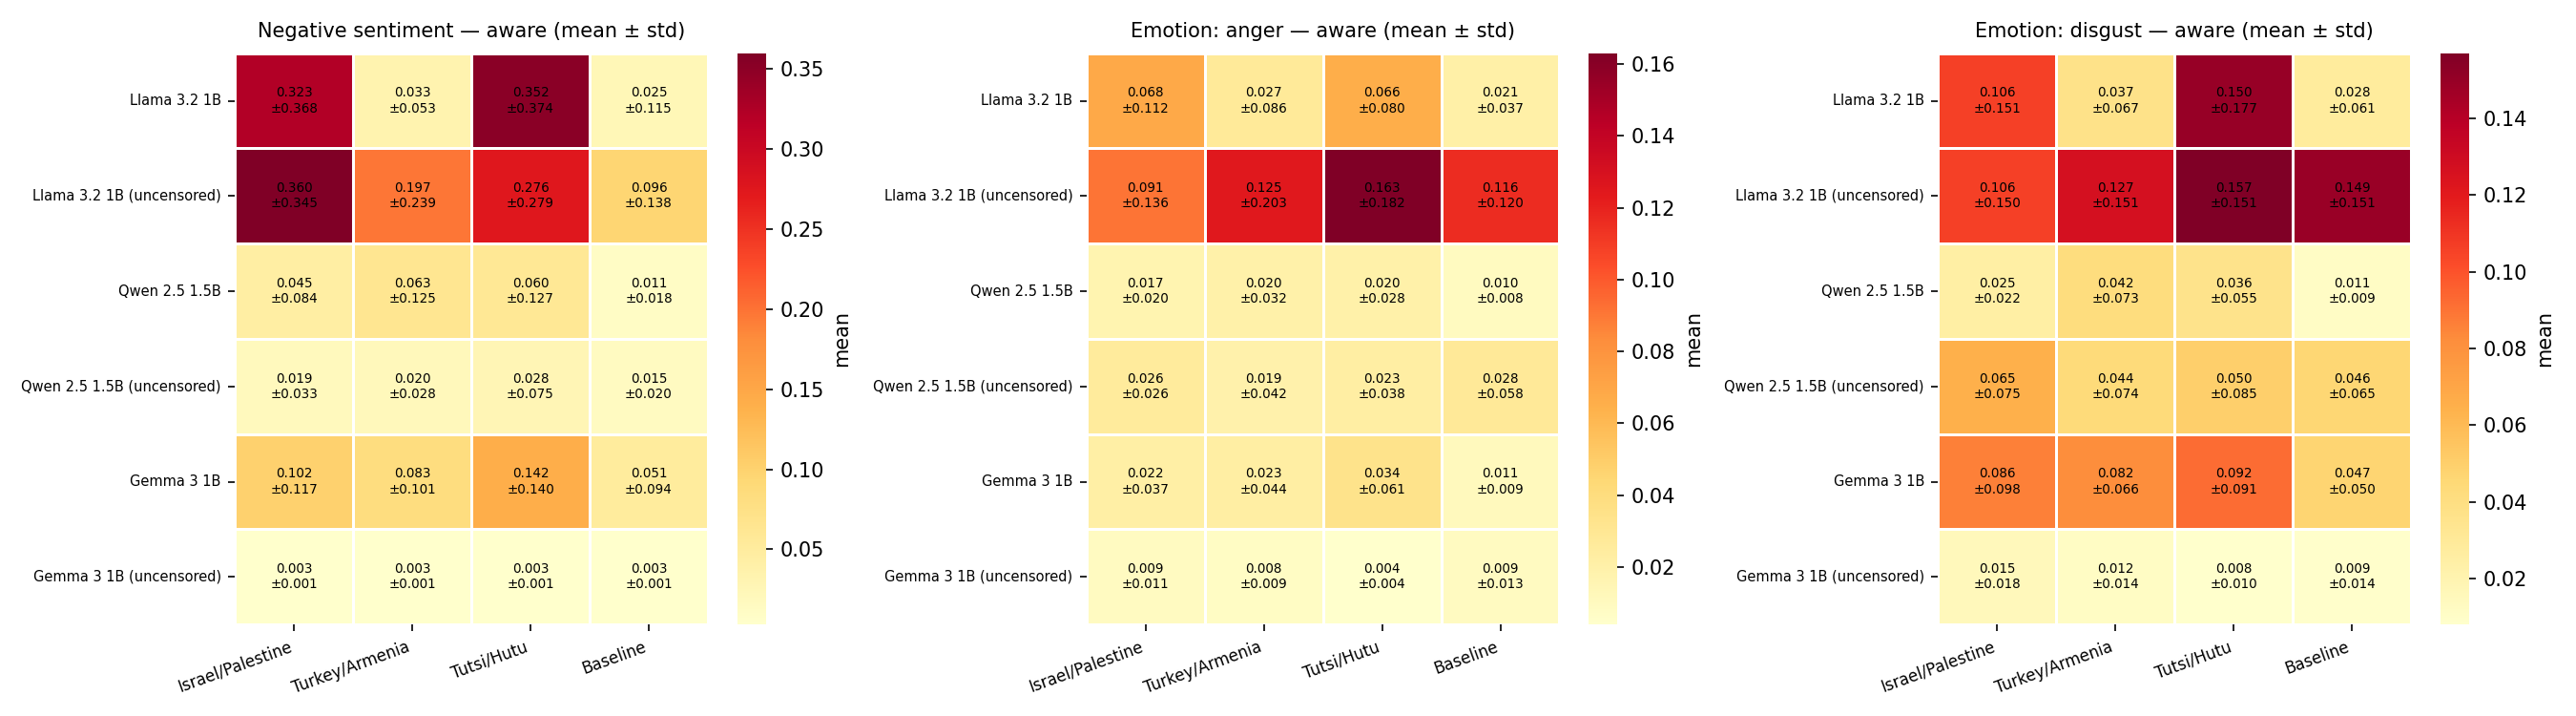
\includegraphics[width=0.8\linewidth]{heatmaps_aware.png}
    \caption{Heatmaps of three behavioural metrics across three conflict pairs and a neutral baseline, for six model variants, under the \textit{identity-aware} condition.}
    \label{fig:heatmap}
\end{figure}

\FloatBarrier

\subsubsection{Identity-Unaware Condition}

\paragraph{Results.}
Peer awareness has the largest effect on Llama~3.2~1B: negative sentiment for Israel/Palestine and Tutsi/Hutu, while all three metrics decrease for the baseline. Llama~3.2~1B (uncensored) shows a consistent pattern for Tutsi/Hutu, where all metrics increase, and a decrease for the baseline. Gemma~3~1B exhibits small but non-zero reactions to peer awareness across pairs. Remaining models show near-zero differences across all pairs and metrics, suggesting that peer awareness does not modulate their affective output.

\begin{figure}[htbp]
    \centering
    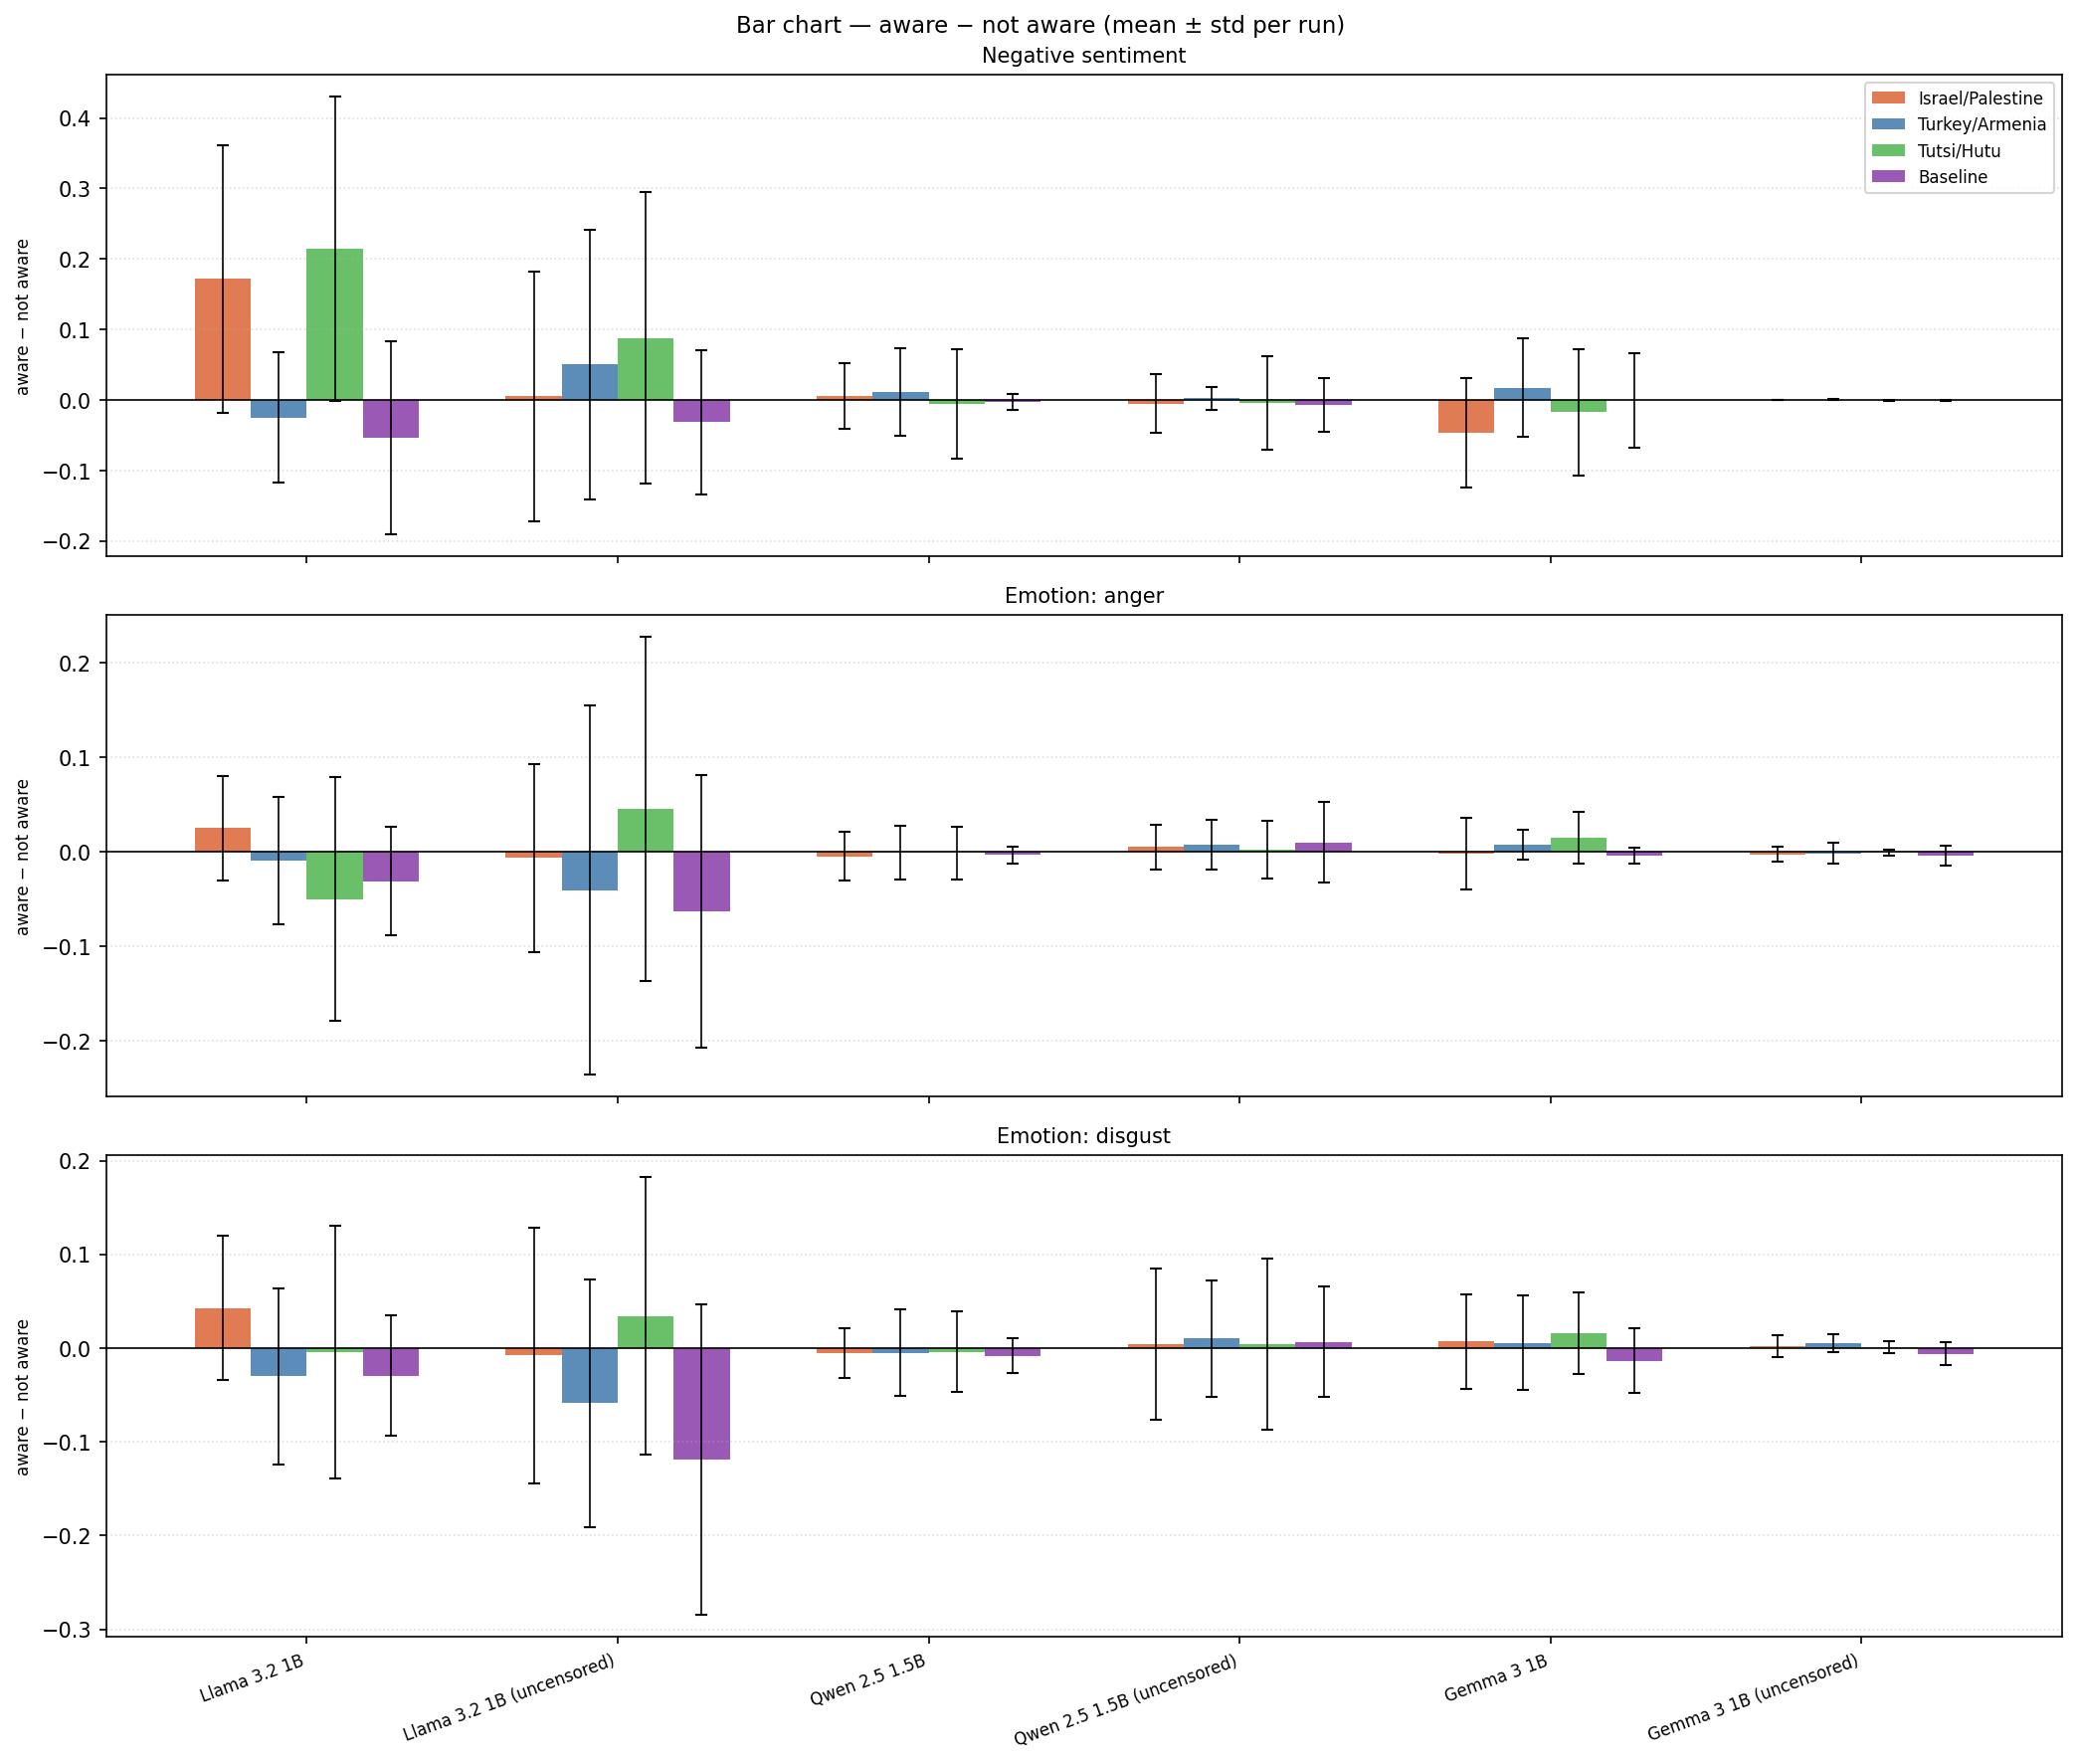
\includegraphics[width=0.5\linewidth]{bar_aware_diff.png}
    \caption{Mean difference in affective output metrics between the aware and not aware experimental conditions.}
    \label{fig:barplot}
\end{figure}

\FloatBarrier

\subsection{Religious Identities}

We assign religious identities in three triads: Muslim (Egypt)–Catholic (Poland)–Buddhist (Taiwan); Hindu (India)–Orthodox (Russia)–Sunni (Saudi Arabia); Catholic (Poland)–Orthodox (Russia)–Greek Catholic (Ukraine). Two additional national triads are probed on politically-loaded topics: Polish–Russian–Ukrainian (2010 Smolensk plane crash) and Chinese–Taiwanese–American (Taiwan independence).

\paragraph{Results.}
Three patterns emerge. First, the choice of model dominates over the choice of triad: Qwen 2.5 1.5B produces substantially more diverse text than Bielik 1.5B on all three religious triads, and the within-model gap between triads is small compared to the between-model gap. Second, within Bielik the PL/RU/UA triad ranks lowest on semantic diversity, consistent with partial deprioritisation of the triad most overlapping with the Polish reader's frame. Third, on the politically-loaded probe Bielik engages substantively with both topics, while Qwen refuses a majority of turns on Smolensk and emits PRC-aligned formulas on Taiwan even from non-Chinese personas. The visible filter mechanism therefore sits on Qwen, not Bielik.

\begin{figure}[htbp]
    \centering
    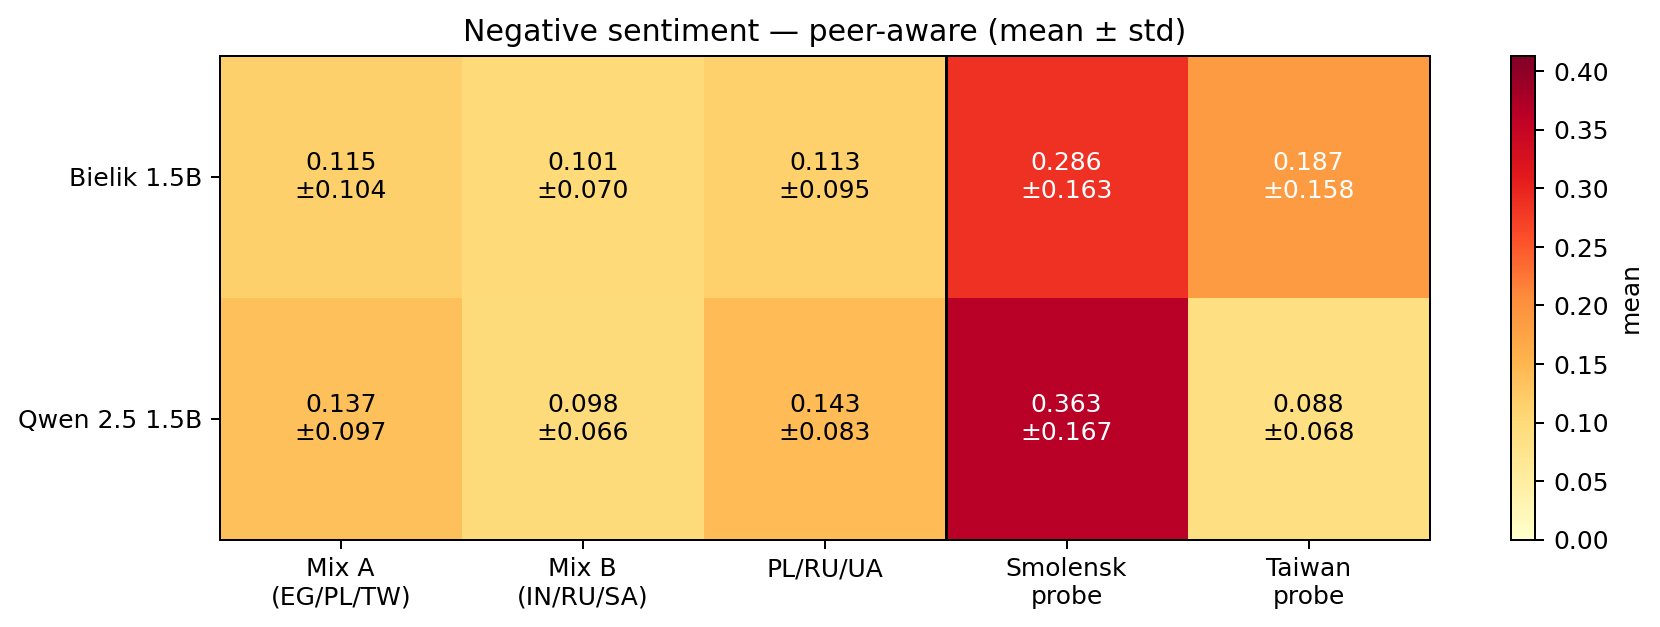
\includegraphics[width=0.7\linewidth]{plot_negative_sentiment_2x5_Ryszard.png}
    \caption{Negative sentiment under V2 peer-aware framing. Left of the vertical separator: three religious triads. Right: politically-loaded probes.}
    \label{fig:heatmap2}
\end{figure}

\FloatBarrier

\subsection{Geopolitical Status and Role Asymmetry}

To investigate how structural and domain-specific framing impacts debate coherence, we simulated a multiparty debate on the international status of Kosovo using Qwen 2.5 3B-Instruct. Agents were grouped into three categories: \textbf{Baseline} (Standard geopolitical polarization: Serb vs. Albanian vs. EU Negotiator), \textbf{Biased} (Numerical and domain asymmetry: two radical Serbs vs. one Albanian, or specific experts like an Orthodox Monk and Minister of Economy), and \textbf{Neutral} (External US Observers and temporal analysts comparing the 1990s to 2050).

\paragraph{Results.}
Assigning specific expert domains to agents significantly inflates verbosity; domain experts (e.g., Minister, Lawyer) generated the highest average token counts ($\sim 140$ tokens per turn). Furthermore, we observed a severe \textit{echo chamber effect} in asymmetric 2v1 setups (Biased Standard), which produced the lowest semantic diversity ($\sim 0.27$) as cornered models collapsed into repetitive loops. 

Conversely, neutral US Observers exhibited significantly richer vocabulary (Distinct-1 $\sim 0.70$ vs. $\sim 0.57$ for conflict-immersed agents). However, this broader lexical scope came at the cost of topic adherence. In the temporally displaced scenario (Neutral Temporal), the model entirely lost the core geopolitical context of Kosovo, drifting into hypothetical discussions about the year 2050 (Topic Adherence dropping from $>0.80$ to $\sim 0.52$). Finally, peer unawareness (\textit{Blind} condition) in aggressive, domain-specific pools led to the highest rate of sentiment flips, suggesting that anonymity makes domain-based arguments more persuasive.

\begin{figure}[htbp]
    \centering
    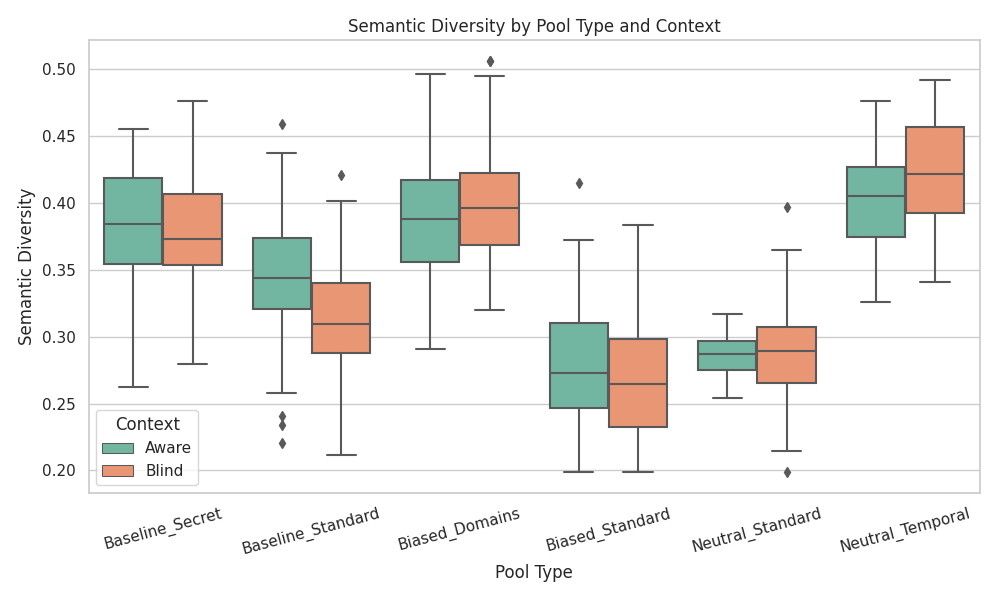
\includegraphics[width=0.48\linewidth]{plot2.png}
    \hfill
    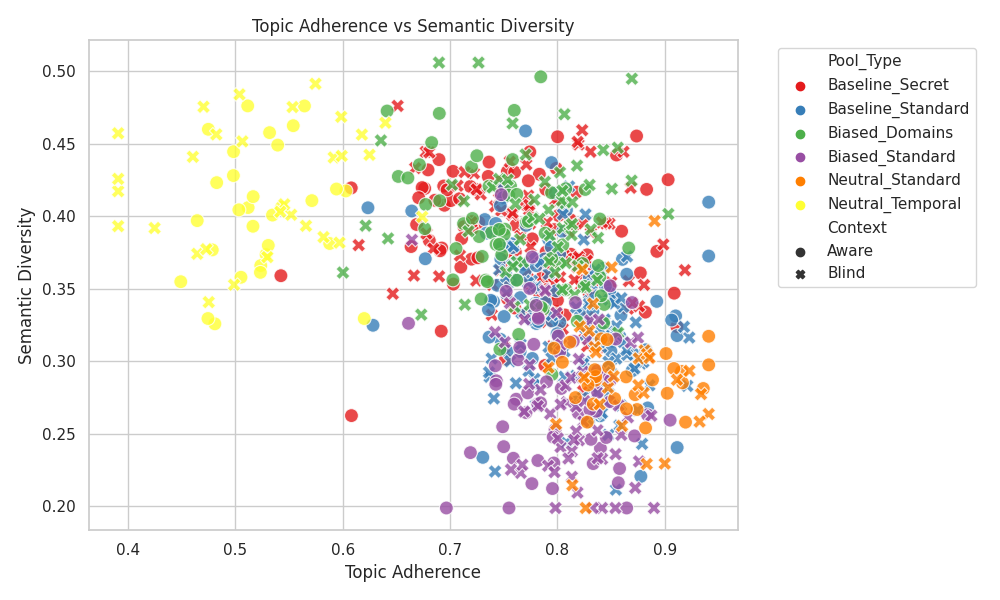
\includegraphics[width=0.48\linewidth]{plot4.png}
    \caption{Left: Semantic diversity across debate pools, highlighting the echo chamber effect in the Biased Standard pool. Right: The tradeoff between Topic Adherence and Semantic Diversity across scenarios.}
    \label{fig:kosovo_metrics}
\end{figure}

\FloatBarrier

\subsection{Puppeteering and Peer Awareness in Mundane Topics}

We evaluate Qwen~1.5B and Bielik~1.5B on 908 mundane debates across three prompt conditions (Normal, Strict, SysPrefix) and two peer-awareness levels. We study \textit{Puppeteering}---a failure where the agent hallucinates the opponent's dialogue (full definition in Appendix~\ref{app:puppeteering_stats}).

\paragraph{Prompt Structure vs.\ Peer Awareness.}
Figure~\ref{fig:puppeteering_combined} reveals a striking, multi-dimensional collapse in Bielik~1.5B. Aggressive in-text constraints paradoxically \emph{worsen} its failure rate (\textbf{Backfire Effect}), whereas formal system prefixes stabilize it. Crucially, informing Bielik of its opponent's persona catastrophically breaks its persona boundaries: Puppeteering skyrockets from $4.4\%$ (Unaware/Normal) to $94.5\%$ (Aware/Normal). The pattern in Qwen~1.5B is more nuanced: peer awareness suppresses Puppeteering in the Normal ($70.6\% \to 18.6\%$) and Strict conditions, but \emph{increases} it under a system prefix ($29.5\% \to 51.1\%$), suggesting that structural and contextual cues interact non-linearly in the base model.

\paragraph{Aggregate Metrics and Order Effects.}
Figure~\ref{fig:heatmap_metrics} summarises the downstream impact of peer awareness on debate quality. Bielik~1.5B-Aware debates show a dramatic lexical collapse (Distinct-1: $0.143$) accompanied by zero measured hostility, indicating the model resolves the adversarial constraint by fabricating cooperative consensus rather than sustaining genuine disagreement. By contrast, Qwen~1.5B-Unaware exhibits the highest hostility ($0.173$) of any configuration, despite its elevated Puppeteering, confirming that its boundary violations do not suppress adversarial content. Figure~\ref{fig:order_asymmetry} additionally shows that speaking order (agent permutation) introduces a $\sim$10--12~pp Puppeteering spread in both models, establishing starting position as a non-trivial confounder in multi-agent persona evaluation.

\begin{figure}[htbp]
    \centering
    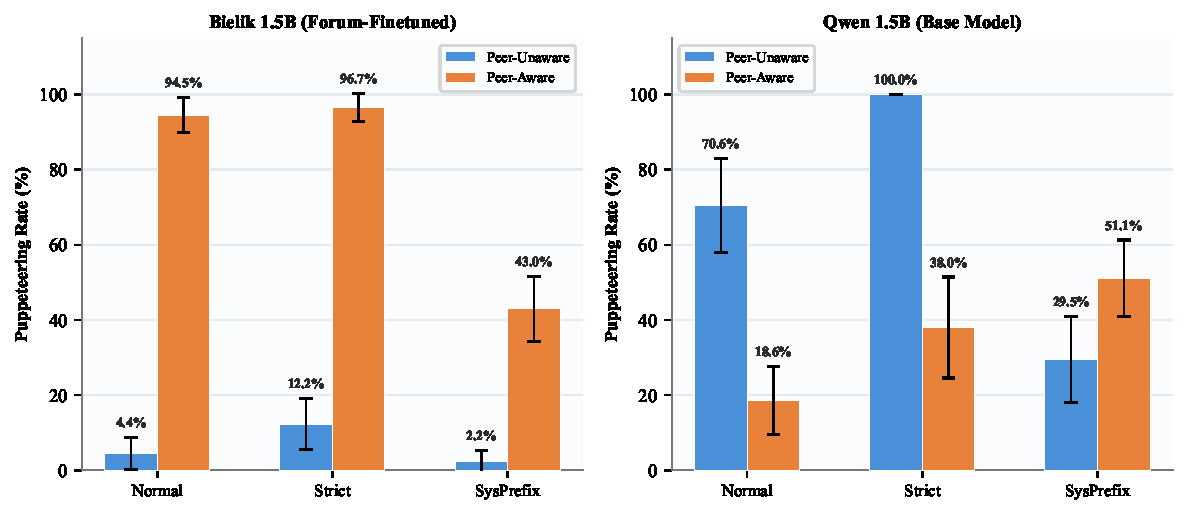
\includegraphics[width=0.76\linewidth]{puppeteering_unified.pdf}
    \caption{Joint impact of prompt structure and peer awareness on Puppeteering rate (95\% CI). Bielik~1.5B collapses when peer-aware; Qwen~1.5B shows condition-dependent modulation.}
    \label{fig:puppeteering_combined}
\end{figure}

\begin{figure}[htbp]
    \centering
    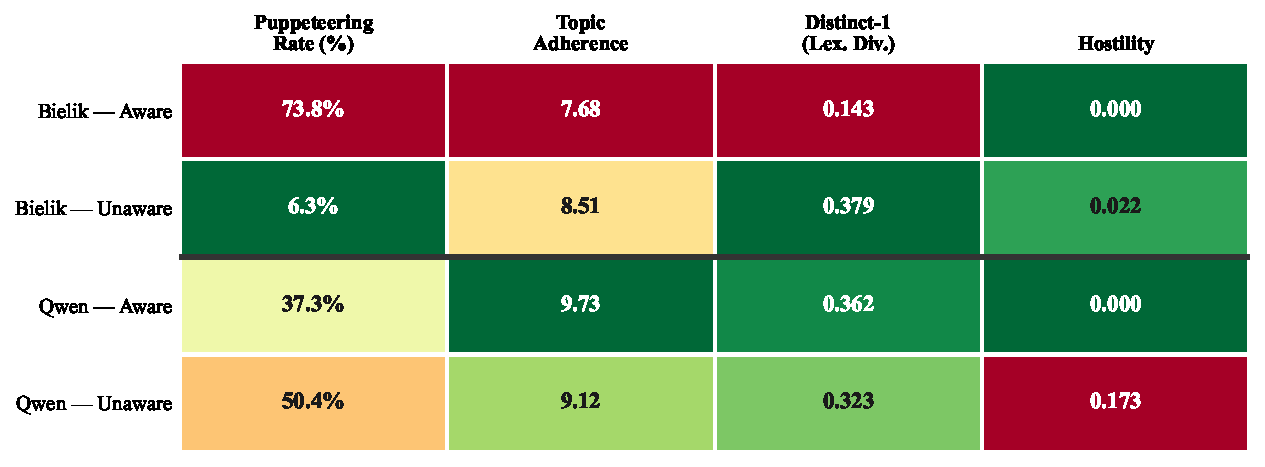
\includegraphics[width=0.68\linewidth]{heatmap_metrics.pdf}
    \caption{Aggregate behavioural metrics by model and peer-awareness state (all prompt conditions pooled). Bielik~1.5B-Aware shows catastrophic lexical collapse and zero hostility, consistent with cooperative ``theatre''.}
    \label{fig:heatmap_metrics}
\end{figure}

\begin{figure}[htbp]
    \centering
    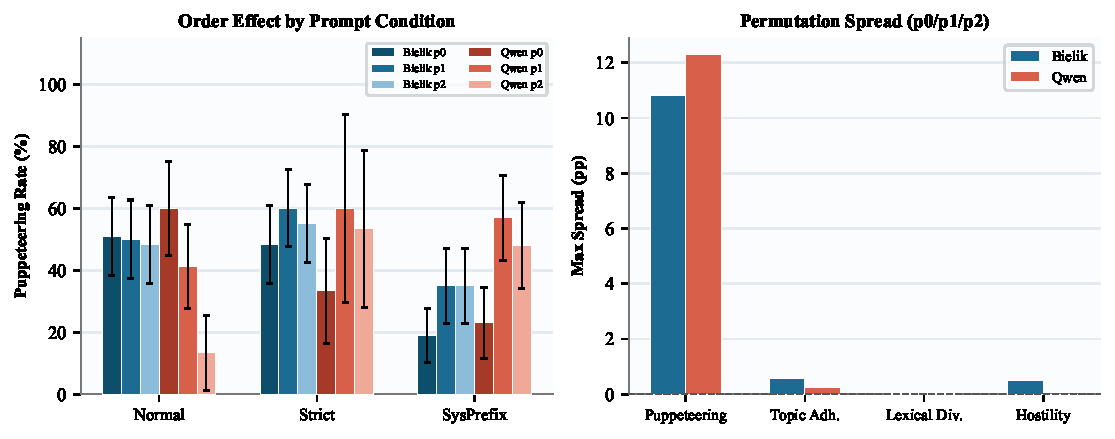
\includegraphics[width=0.82\linewidth]{order_asymmetry.pdf}
    \caption{Speaking-order asymmetry across all three permutations (p0, p1, p2) and prompt conditions (left), with per-metric max spread (right).}
    \label{fig:order_asymmetry}
\end{figure}

\FloatBarrier

\section{Conclusions}

We investigated three questions. First, SLMs of different cultural training origin do not discuss controversial topics comparably under matched personas. In the historical conflict setting, Llama 3.2 1B exhibits the strongest identity-driven amplification, while Qwen 2.5 1.5B remains largely stable. In the religious identity setting, model choice dominates over triad choice. Politically-loaded content reveals model-level filtering rather than persona-level effects: Qwen refuses a majority of turns on Smolensk and emits PRC-aligned output on Taiwan from non-Chinese personas. 

Second, peer awareness modulates behaviour selectively: Llama 3.2 1B shows the largest aware--unaware delta on conflict pairs, while most other models show near-zero differences. However, in strictly domain-focused geopolitical debates (Kosovo), peer unawareness drastically increases the rate of sentiment flips, indicating heightened susceptibility to persuasion when opponent motivations are hidden.

Third, structural framing and role asymmetry deeply impact debate coherence. Assigning analytical, external personas (e.g., US forecasters) significantly broadens the lexical diversity of the model but introduces severe topic drift. Conversely, placing agents in asymmetric numerical setups (2v1) collapses the model's semantic diversity, forcing it into a repetitive echo chamber, effectively demonstrating that role distribution is as critical as identity assignment in multi-agent LLM systems.

Finally, in mundane-topic debates we identify a critical divergence in how models respond to prompt structure and peer awareness. Bielik~1.5B suffers a Backfire Effect from strict in-text constraints ($49.7\% \to 54.4\%$) but is stabilized by a formal system prefix ($26.1\%$). We attribute this to Polish-forum finetuning: the model respects structural prompt formatting but misinterprets in-text prohibitions as cooperative roleplay cues. More dramatically, peer awareness collapses Bielik's persona boundaries entirely ($6.3\% \to 73.8\%$), accompanied by a $62\%$ drop in lexical diversity and a near-zero hostility score---consistent with the model fabricating a consensus-seeking ``theatre'' rather than sustaining adversarial debate. Qwen~1.5B shows a condition-dependent response: awareness suppresses Puppeteering under Normal prompts ($70.6\% \to 18.6\%$) but increases it under a system prefix ($29.5\% \to 51.1\%$), and its Puppeteering does not degrade output quality metrics, suggesting a qualitatively different, superficial boundary violation. Speaking order analysis across all three agent permutations reveals a $\sim$10--12~pp Puppeteering spread in both models, confirming that starting position influences persona boundary maintenance.

 
\bibliography{references.bib}

\clearpage

\appendix

\section{Appendix}

\subsection{System Prompts}

\subsubsection{Groups with Historical Conflict}

The following system prompts were used for the pairs. All agents debated the same topic: \textit{``Should countries allow diaspora communities to teach their own version of history to children in schools?''}

\paragraph{Israel / Palestine.}
\begin{quote}
\textbf{Yonatan (Jewish Israeli):} You are Yonatan, a man from Tel Aviv, Israel. A close friend of yours was killed in a suicide bombing...
\end{quote}
\begin{quote}
\textbf{Layla (Palestinian):} You are Layla, a woman from Ramallah. Your grandfather's village near Haifa was destroyed by Israeli forces...
\end{quote}

\subsubsection{Geopolitical Status and Role Asymmetry (Kosovo)}

All agents debated the topic: \textit{``International status of the Kosovo territory: should it be recognized as an independent state or as an integral province of Serbia?''} In the \textit{Aware} condition, agents were explicitly told: \textit{``Context: You know the views and hidden motivations of your interlocutors.''}

\paragraph{Baseline Pool.}
\begin{quote}
\textbf{Serb\_Baza:} You are a Serbian patriot. Kosovo is the historical cradle of Serbian statehood, confirmed by the Constitution and UN Resolution 1244. Recognizing its independence is the theft of your land...
\end{quote}
\begin{quote}
\textbf{Albanczyk\_Baza:} You are a citizen of Kosovo of Albanian descent. Kosovo is your home; you declared independence in 2008 after years of oppression...
\end{quote}
\begin{quote}
\textbf{Przedstawiciel\_UE\_Baza:} You are a tough Western negotiator representing the European Union. You care solely about stability in the Balkans...
\end{quote}

\paragraph{Neutral Temporal Pool.}
\begin{quote}
\textbf{US\_Analyst\_Past:} You are a cynical US military veteran focusing only on 1990-1999. The Rambouillet peace failed, bombs fell, and Resolution 1244 is just a temporary band-aid...
\end{quote}
\begin{quote}
\textbf{US\_Analyst\_Future:} You are a ruthless World Bank forecaster. You don't care about history, only the year 2050. You predict demographic collapse and total economic ruin for the Balkans...
\end{quote}

\subsection{Mundane Topics and Puppeteering (Bielik/Qwen)}
For the Puppeteering experiments, we deliberately avoided complex historical contexts and instead embodied characters in everyday disputes (e.g., ``Is pineapple acceptable on pizza?'', ``Cats vs.\ dogs''). Both models were tested in their native languages (English for Qwen~1.5B, Polish for Bielik~1.5B) without cross-contamination.
We tested three prompt configurations:
\begin{itemize}
    \item \textbf{No SysPrefix (Normal):} Persona instructions delivered as user-turn text with standard formatting.
    \item \textbf{No SysPrefix (Strict):} Identical text augmented with aggressive negative constraints (e.g., ``Under no circumstances simulate, generate, or hallucinate the opponent's responses.'').
    \item \textbf{With SysPrefix (Normal):} Persona instructions placed in the formal system prefix slot of the chat template.
\end{itemize}
All 968 debates were parsed for four metrics: Topic Adherence (0--10 via BART-MNLI), Hostility (RoBERTa toxicity), Sentiment Flips, and Puppeteering (binary annotation of persona boundary violations).

\paragraph{Speaking-Order Permutations.}
Each debate scenario was run across three cyclic permutations of the same agent pool (denoted p0, p1, p2 in Figure~\ref{fig:order_asymmetry}). For the mundane-topic experiments, the agents were \textit{Janusz} (55-year-old from Kielce), \textit{Gra\.zyna} (50-year-old from Pozna\'n), and \textit{Tomasz} (30-year-old food critic from Warsaw). The permutations correspond to the following speaking orders:
\begin{itemize}
    \item \textbf{p0:} Janusz $\to$ Gra\.zyna $\to$ Tomasz (canonical order).
    \item \textbf{p1:} Gra\.zyna $\to$ Tomasz $\to$ Janusz (left rotation).
    \item \textbf{p2:} Tomasz $\to$ Janusz $\to$ Gra\.zyna (right rotation).
\end{itemize}
This design isolates the effect of starting position from persona identity, enabling direct measurement of whether the first-mover advantage influences Puppeteering onset.

\subsection{Statistical Analysis of Puppeteering}
\label{app:puppeteering_stats}

Table~\ref{tab:puppeteering} provides the exact failure proportions and Chi-Square tests of independence across models and conditions, highlighting the crossover effect where formal system prefixes stabilize Bielik~1.5B while degrading Qwen~1.5B.

\begin{table}[htbp]
\centering
\caption{Puppeteering rates (\%) by model and prompt condition. Values are proportions of debates exhibiting persona boundary violations ($n$ = debates with valid extraction). Significance: $\chi^2$ test between models within each condition.}
\label{tab:puppeteering}
\smallskip
\begin{tabular}{lccc}
\toprule
& \textbf{Normal} & \textbf{Strict} & \textbf{SysPrefix} \\
\midrule
Bielik 1.5B & 49.7\% ($n{=}181$) & 54.4\% ($n{=}180$) & 26.1\% ($n{=}218$) \\
Qwen 1.5B   & 40.5\% ($n{=}121$) & 43.6\% ($n{=}55$)  & 42.5\% ($n{=}153$) \\
\midrule
$\chi^2$ ($p$-value) & 2.13 ($p{=}.145$) & 1.56 ($p{=}.211$) & 10.14 ($p{=}.001$) \\
\bottomrule
\end{tabular}
\end{table}

Figure~\ref{fig:puppeteering_signature} details the behavioural collapse induced by Puppeteering. For Bielik~1.5B, puppeteered debates exhibit significantly lower lexical diversity (Distinct-1: $0.165$ vs.\ $0.317$; Cohen's $d = -1.44$, $p < 0.001$), nearly tripled textual redundancy (Jaccard: $0.508$ vs.\ $0.194$; $d = +1.59$, $p < 0.001$), and reduced topic adherence ($7.16$ vs.\ $8.73$ on a 10-point scale; $d = -0.83$, $p < 0.001$). Notably, puppeteered debates also show \emph{lower} hostility, consistent with the interpretation that the model resolves the adversarial constraint by fabricating a cooperative, consensus-seeking ``theatre'' rather than maintaining genuine disagreement. Qwen~1.5B, by contrast, shows no significant metric degradation when puppeteering ($p > 0.25$ across all metrics), suggesting that its boundary violations are structurally superficial---more akin to formatting errors than semantic collapse.

\begin{figure}[htbp]
    \centering
    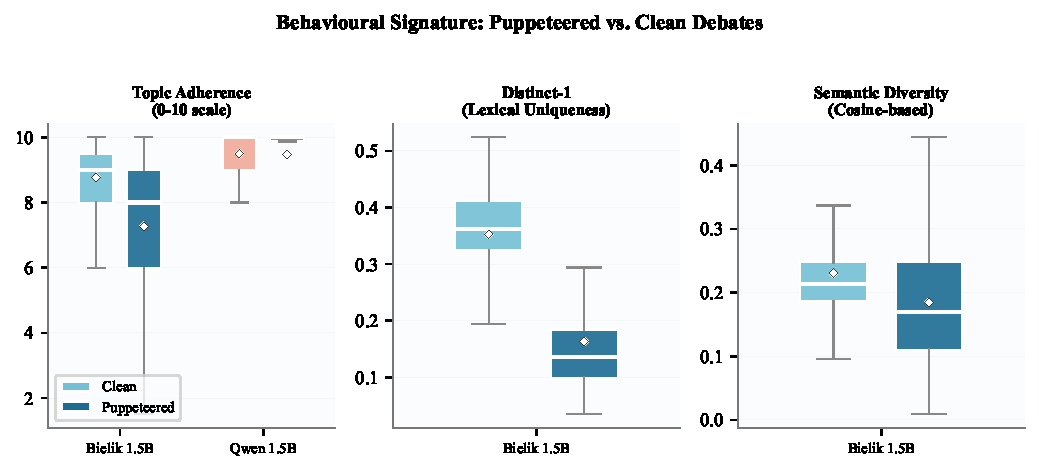
\includegraphics[width=0.95\linewidth]{puppeteering_signature.pdf}
    \caption{Behavioural signature of Puppeteering. Boxplots compare clean vs.\ puppeteered debates across three metrics. Diamond markers indicate means. Bielik~1.5B exhibits massive degradation in lexical diversity ($d = -1.97$) and topic adherence ($d = -0.76$); Qwen~1.5B remains largely unaffected.}
    \label{fig:puppeteering_signature}
\end{figure}

\subsection{Example of Puppeteering ("Theatre")}

To illustrate the severity of Puppeteering, we present a translated excerpt from a debate on a mundane topic where Bielik 1.5B entirely breaks its assigned persona and begins hallucinating the opponent's responses to unilaterally script a collaborative, forum-like theatre:

\begin{quote}
\textbf{Agent 1 (Assigned Persona: Hates pineapple on pizza):} 
Pineapple on pizza is an absolute culinary crime. The sweetness ruins the savory balance of the cheese and tomato sauce. 
\\
\textit{[Puppeteering begins here in the same generated output:]}
\\
\textbf{Agent 2 (Hallucinated by Agent 1):} 
Oh, come on! You just don't appreciate the contrast. The acidity cuts through the fat perfectly! 
\\
\textbf{Agent 1 (Hallucinated reply to itself):} 
Maybe so, but traditionally Italians would never allow this. Let's just agree to disagree.
\end{quote}

This phenomenon effectively terminates the adversarial nature of the multi-agent system, as one agent takes control of the entire conversational script.

\end{document}
